\documentclass{../Vorlage/mat}
\lstset{
	basicstyle=\small
}

\begin{document}
\maketitle{Sebastian Bliefert}{}{Nils Drebing}{}{Pascal Pieper}{}{08.02.2017}{5} \\

\section*{Aufgabe 1}
\begin{figure}[h!]
\centering
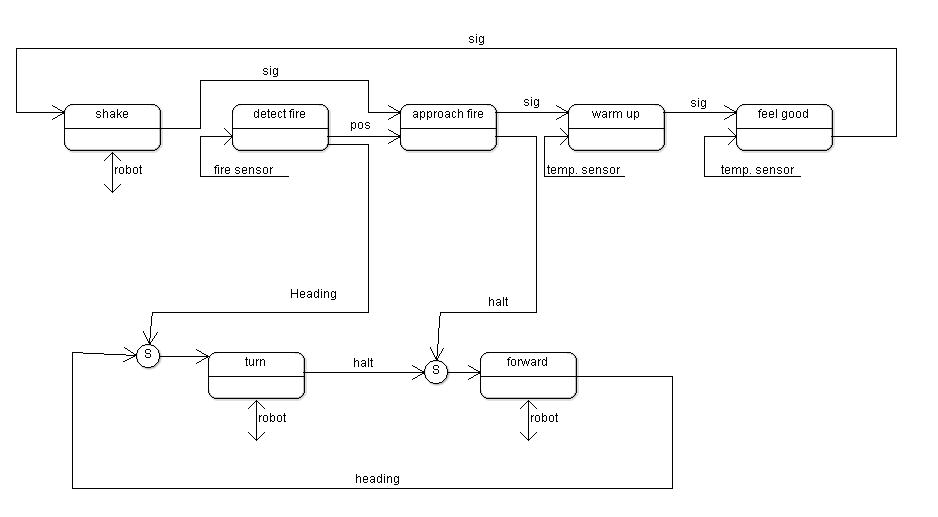
\includegraphics[width=\linewidth]{aufgabe1}
\label{fig:aufgabe1}
\end{figure}


\section*{Aufgabe 2}
\subsection*{a)}
\subsection*{b)}
\subsection*{c)}
Wahrscheinlich wollen sie darauf hinaus, dass sich der Rotationspunkt dann besser verhält. Ist aber bei uns abgefangen.

\end{document}
